% Manuscript prepared for Electronics (MDPI), Artificial Intelligence section.
% Special Issue: Trustworthy AI for Large Models and Security Systems.
% Compile inside the official MDPI LaTeX template.
% Before submission, verify the journal option against the current MDPI template
% and complete all author declarations in the submission system.
\documentclass[electronics,article,submit,pdftex,moreauthors]{Definitions/mdpi}

\Title{Information Leakage from Token-Length Traces in Streaming LLMs: Cross-Model Reconstruction and Defense Evaluation}
\Author{Paweł Augustynowicz $^{1,*}$ and Szymon Jędrzejczak $^{1,*}$}
\AuthorNames{Paweł Augustynowicz and Szymon Jędrzejczak}
\address[1]{Faculty of Cybernetics, Military University of Technology, gen. Sylwestra Kaliskiego 2, 00-908 Warsaw, Poland; pawel.augustynowicz@wat.edu.pl (P.A.); szymon.jedrzejczak@wat.edu.pl (S.J.)}
\corres{Correspondence: pawel.augustynowicz@wat.edu.pl (P.A.); szymon.jedrzejczak@wat.edu.pl (S.J.)}

\pubvolume{1}
\issuenum{1}
\articlenumber{0}
\pubyear{2026}
\copyrightyear{2026}
\datereceived{}
\daterevised{}
\dateaccepted{}
\datepublished{}

\usepackage{booktabs}
\usepackage{multirow}
\usepackage{graphicx}
\usepackage{array}
\usepackage{longtable}
\usepackage{tabularx}
\usepackage{threeparttable}
\usepackage{amsmath}
\usepackage{enumitem}
\usepackage{placeins}
\usepackage{tikz}
\usetikzlibrary{arrows.meta,positioning,shapes.geometric,fit}
\usepackage{pgfplots}
\pgfplotsset{compat=1.18}
\setlength{\headheight}{24pt}

\abstract{Streaming large language model (LLM) services can expose message-size metadata even when payloads are encrypted. We evaluate a fixed T5-based reconstructor in an instrumented, application-layer setting, using 300 aligned prompts for each of seven open-weight models and a 512-token generation limit. Saved term-frequency cosine scores (\texorpdfstring{$\phi$}{phi}) range from 0.030 to 0.568, with five models at 0.517--0.568. These are historical pipeline scores: an audit found that the archived line-based collector can discard token newline bytes, while the exact historical reconstruction inputs are unavailable in the supplied artifacts. References from TinyLlama and Phi-3.5-mini also exhibit missing word boundaries; those two series are retained as apparatus diagnostics and do not establish poor transfer to normally decoded responses. Victim responses reached end-of-sequence before the token limit in 0--65.7\% of cases. In separate 96-token pilots with 30 prompts per model, ordered logged traces exceeded shuffled, constant, and cross-prompt controls by 0.046--0.196 in mean \texorpdfstring{$\phi$}{phi}. These controls remove only selected trace features and do not isolate a pure language-prior baseline. Five framing transformations reduced frozen-reconstructor scores by 35.0--90.3\% in those pilots. A 512-token study with five decoder seeds and a prompt-disjoint maximum-a-posteriori (MAP) inverse included 3300 reconstructions; adaptation recovered much of the score lost under bucketing and batching. This study decoded only the first heuristic segment and scored it against the entire saved response. Both T5 input and output were limited to 80 tokens, so changes in segmentation and retained input also affect these comparisons. The results characterize a bounded reconstruction pipeline, rather than semantic disclosure, intrinsic model vulnerability, or attack success on encrypted transport traffic.}

\keyword{large language models; information leakage; side-channel analysis; server-sent events; traffic analysis; token-length traces; text reconstruction; privacy}

\begin{document}

\section{Introduction}
Interactive large language model (LLM) services stream partial responses to reduce latency. One implementation uses Server-Sent Events (SSE), with generated text carried in application events. Encryption hides the event contents but not necessarily the shape of the communication. If application-event boundaries or correlated record sizes are observable, a sequence of lengths can reveal properties of the underlying tokens.

This paper separates trace-based reconstruction from the recovery of a trace from encrypted production traffic. The intended laboratory observable is the ordered UTF-8 byte length of each token emitted by an instrumented service, before transport processing. This abstraction removes segmentation by HTTP and Transport Layer Security (TLS), buffering, retransmission, and multiplexing from the experiment. The implementation audit in Section~\ref{sec:measurement-audit}, however, identifies a mismatch between logged token lengths and the archived line-based collection path. We therefore distinguish the intended oracle from the saved historical pipeline results and from experiments that read token lengths directly from logs. No experiment here establishes passive extraction of event boundaries from encrypted traffic.

Building on Weiss \emph{et al.}, who reconstructed streamed responses from token-length patterns using a T5-based inversion pipeline~\cite{weiss2024prompt}, we examine one fixed reconstructor across open-weight victim models. Partial trace ablations assess its sensitivity to ordered lengths, and framing transformations test its response without retraining. Cross-model interpretation is conditional on collection provenance and reference decoding; the TinyLlama and Phi-3.5-mini series are treated as apparatus diagnostics.

The study addresses three research questions:
\begin{enumerate}[label=\textbf{RQ\arabic*:},leftmargin=4.2em,labelwidth=3.2em,labelsep=0.6em]
    \item Do ordered logged lengths improve lexical scores over controls that shuffle lengths, replace them with a constant, or use another prompt's trace?
    \item How do saved reconstruction scores differ across seven victim-model runs, and which comparisons remain interpretable after auditing collection and reference decoding?
    \item How do bucketing, fixed-width units, batching, and randomized padding affect the evaluated pipeline, protected-payload size, and frame count, and how does a prompt-disjoint maximum-a-posteriori (MAP) inverse change its scores?
\end{enumerate}

The contribution is an artifact-backed evaluation of a fixed reconstruction pipeline. It provides a seven-run, prompt-aligned archive with descriptive score comparisons; an audit of observation and detokenization limitations; two-model pilots of partial trace ablations and five framing configurations; and a five-seed MAP-inverse evaluation on responses generated with a 512-token budget. The pilots and MAP study use different reconstruction scopes, so their baselines are not interchangeable. Code, prompts, saved outputs, and analysis files are organized at \url{https://github.com/jackaugustyn/LLeakM}. The historical reproducibility manifest and a separate revision snapshot have distinct roles, as detailed in Appendix~\ref{app:runs}.

\section{Related Work}
Side-channel attacks infer sensitive information from indirect observables such as timing and message size. Classical timing attacks showed that implementation-level leakage can defeat cryptographic protection without recovering plaintext directly~\cite{kocher1996timing}. Encrypted network applications likewise leak through packet sizes and timing. Keystroke inference, web-application traffic analysis, and website fingerprinting demonstrate that encryption does not hide communication shape~\cite{song2001timing,chen2010sidechannel,cai2012touching,sirinam2018deep}.

Traffic-analysis defenses transform that shape through padding, morphing, batching, or cover traffic. Traffic morphing attempts to make one traffic class resemble another, while subsequent studies show that efficient countermeasures may retain exploitable structure or impose substantial overhead~\cite{wright2009morphing,dyer2012peekaboo}. For this reason, defense effectiveness should be evaluated by reporting both the leakage that remains and the resulting bandwidth and latency overhead, rather than by treating padding as either fully protective or ineffective.

For generative AI, Weiss \emph{et al.} introduced T5-based sequence-to-text inversion and reported accurate reconstruction for 27\% of responses and topic inference for 53\% in their evaluated setting~\cite{weiss2024prompt}. Li \emph{et al.} subsequently studied API outputs that merge several tokens into one observable unit and showed that aggregation does not remove the side channel~\cite{li2026length}. Whisper Leak instead infers prompt topics from packet-size and timing patterns in encrypted LLM traffic~\cite{whisperleak2025}. Those studies address stronger deployment-facing threat models. The present work narrows the observation layer to ask a different question: how a fixed reconstructor transfers across victim models once a token-granular length trace is available, and how simple transformations affect that same reconstructor.

The reconstruction pipeline uses T5-style text-to-text transformers~\cite{raffel2020exploring}. Evaluation combines a reference-normalized Levenshtein distance~\cite{levenshtein1966binary}, ROUGE precision~\cite{lin2004rouge}, and one fixed term-frequency cosine score $\phi$. These are lexical measures. They should not be read as semantic correctness or disclosure of a usable answer.

\section{Materials and Methods}
\subsection{Threat Model and Objective}
We evaluate a length-only reconstructor for an instrumented LLM service. The intended observation is the ordered byte length of each emitted token payload, with no access to the generating prompt, token identities, or victim-model internals. This is an application-layer length-oracle abstraction: it does not recover event boundaries from TLS, HTTP/2, or QUIC traffic. The retained cross-model campaign and the later log-based experiments use different collection paths. Section~\ref{sec:measurement-audit} identifies the resulting measurement and reference-text limitations; the cross-model scores are therefore reported as historical apparatus measurements rather than a validated ranking of ordinary model responses.

The objective is to characterize lexical reconstruction in this controlled apparatus and the response of a fixed reconstructor to length transformations. The experiments capture per-token traces, reconstruct text from length sequences, and compare the reconstructions with the stored emitted responses. Prompts are used to generate those responses and are not supplied to the reconstructor. Figure~\ref{fig:threat_model} shows the intended information flow.

\subsection{Information-Theoretic Interpretation}
Let $R$ denote the stored emitted response and let $X=(L_1,\ldots,L_T)$ denote its ordered token-payload length trace in the idealized laboratory model. When a defense is applied, $X$ is transformed into the observable trace $Z=g(X,N)$, where $N$ is independent transformation randomness. The attacker produces $\widehat{R}=A(Z,U)$ using independent decoder randomness $U$. Conditional on a fixed fitted attacker, these relationships form the following Markov chain:
\begin{equation}
R \longrightarrow X \longrightarrow Z \longrightarrow \widehat{R}.
\end{equation}
According to the data-processing inequality,
\begin{equation}
I(R;\widehat{R}) \leq I(R;Z) \leq I(R;X).
\end{equation}
Neither processing stage increases mutual information about $R$ under these assumptions. The empirical controls are partial trace ablations: they preserve response-dependent features such as trace length, the length histogram, or mean length. A score advantage over an ablation indicates sensitivity to the altered features, but does not isolate all trace information from the decoder's language prior. The lexical score $\phi$ does not estimate mutual information, and its reduction for a fixed attacker does not measure defended-channel capacity.

\begin{figure*}[ht]
\centering
\resizebox{\textwidth}{!}{%
\begin{tikzpicture}[node distance=10mm and 12mm,>=Latex,
box/.style={draw,rounded corners,align=center,minimum height=10mm,minimum width=31mm,fill=blue!5},
obs/.style={draw,dashed,rounded corners,align=center,minimum height=10mm,minimum width=35mm,fill=orange!10}]
\node[box] (user) {Prompt corpus};
\node[box,right=of user] (victim) {Victim LLM\\instrumented SSE service};
\node[box,right=of victim] (stream) {One token per\\application event};
\node[obs,below=of stream] (oracle) {Intended observation:\\ordered payload byte lengths};
\node[box,left=of oracle] (attacker) {Fixed T5\\reconstructor};
\node[box,left=of attacker] (score) {Lexical recovery\\metrics};
\draw[->] (user)--(victim);
\draw[->] (victim)--(stream);
\draw[->] (stream)--(oracle);
\draw[->] (oracle)--(attacker);
\draw[->] (attacker)--(score);
\node[draw,dotted,fit=(stream)(oracle),inner sep=4mm,label=below:{Application-layer length oracle; TLS extraction is out of scope}] {};
\end{tikzpicture}%
}
\caption{Intended threat model. The attacker receives application-layer lengths without the prompt or token identities. The collection-path discrepancy is documented in Section~\ref{sec:measurement-audit}; passive recovery of event boundaries from encrypted transport is outside the experiment.}
\label{fig:threat_model}
\end{figure*}

\subsection{Streaming Harness and Trace Collection}
The historical harness emitted one separately decoded token payload per streaming write. Each write had the SSE-like byte serialization \texttt{data: \textless token\textgreater\textbackslash n\textbackslash n}; stream termination used \texttt{data: [DONE]\textbackslash n\textbackslash n}. Token text, token UTF-8 length, serialized-write UTF-8 length, and relative timestamp were logged. Per-run metadata included the model identifier, decoding parameters, prompt, concatenated emitted response, and token count. Raw newline characters within token text were not escaped, so a streaming write is not necessarily a single valid SSE data event. The reconstruction input used lengths only.

For the logged serialization, the payload length satisfies
\begin{equation}
L^{\mathrm{log}}_t = L^{\mathrm{write}}_t - 8,
\end{equation}
where the eight bytes are the prefix \texttt{data: } and suffix \texttt{\textbackslash n\textbackslash n}. This identity concerns the complete emitted byte string, including any newline bytes inside the payload. The terminal \texttt{[DONE]} write is excluded. The control pilots, defense pilots, and MAP study read \texttt{token\_utf8\_len} directly from the generation logs. The archived source audited for the primary campaign instead called a line-based collector before subtracting eight bytes.

\subsection{Measurement and Reference-Text Audit}\label{sec:measurement-audit}
The archived collector used \texttt{requests.iter\_lines()} to split the incoming stream. Its implementation in \texttt{run\_validation.py} discarded empty lines and appended two newline bytes to each remaining line. Its inferred vector $X^{\mathrm{col}}$ therefore need not equal the logged payload vector $X^{\mathrm{log}}$. For example, the payload \texttt{:\textbackslash n\textbackslash n} has three bytes, but replay of this collector gives an inferred length of one. Replaying that implementation on the retained logs changes 2073 of 2100 vectors and the number of heuristic segments in 764 samples, despite matching the number of collected units in every sample. These are preprocessing-replay results, not archived historical T5 inputs. The exact primary input vectors and their binding to the collector version are unavailable in the supplied artifacts, so the replay does not establish which historical reconstructions were affected or how their scores would change. The reported primary scores are preserved; they must not be interpreted as results from a newly corrected common observation pipeline.

A separate audit concerns reference text. The historical harness decoded each token independently and concatenated the strings, without a demonstrated equivalence to decoding the complete token sequence. Of the stored references, 299/300 TinyLlama responses and 162/300 Phi-3.5-mini responses contain no ASCII space. This affects word-based evaluation and potentially the corresponding byte-length trace. Those two series are retained as apparatus diagnostics, not evidence of weak transfer on normally detokenized model responses. The observed counts do not determine how much of the score difference detokenization explains. Reliable replacement references require original token-sequence provenance or new generation with validated detokenization; inserting spaces heuristically would not recover ground truth.

The audit uses existing logs, recorded outputs, and local tokenizer resources without new victim generation or T5 inference. Its scripts and detailed outputs are retained under \texttt{reviews/ars\_electronics\_20261031/phase1\_panel/} in the accompanying repository. Subsequent code repairs replace line parsing with a validated log-length oracle and check received byte totals; this remains an instrumented observation, not passive transport extraction. The revised harness checks that context-aware token fragments concatenate to the full decoded response and records generated token IDs and provenance. These repairs do not retroactively validate archived outputs. Revalidation artifacts, including 2100 verified logged length vectors and separate reconstruction-run status files, are stored under \path{experiment_validation/revalidation_20261031/}; incomplete runs do not enter the manuscript's tables.

\subsection{Reconstruction Pipeline}
The inversion pipeline follows the sequence-to-text procedure introduced by Weiss \emph{et al.}~\cite{weiss2024prompt}. It first splits a length vector at observations equal to one and merges short chunks using a ten-unit minimum, with an additional list-boundary heuristic. These are heuristic segments rather than verified sentences. The first segment is decoded using \texttt{royweiss1/T5\_FirstSentences}; later segments use \texttt{royweiss1/T5\_MiddleSentences} with preceding reconstructed context. Multiple decoding candidates are ranked by the transition log-probability sum.

For defense experiments, the order is length transformation, optional MAP inversion, heuristic segmentation, serialization of each segment as underscore-prefixed integers, T5 tokenization, input truncation, and decoding. The encoder input is limited to 80 T5 tokens, including the instruction prefix and any preceding context; generation also uses \texttt{max\_length}=80. These limits are distinct from the victim's 96- or 512-token generation budget. One length value need not occupy one T5 token: for example, \texttt{\_32} occupies two tokens in the audited tokenizer. Changing the length values can therefore change both segmentation and the amount of trace retained by the encoder. Section~\ref{sec:robustness-methods} reports the audited coverage of the first segment in the MAP experiment.

The reconstruction design is conditional rather than purely tokenwise. Instead of recovering each token independently, it maps length patterns into coherent text spans and uses context to improve linguistic plausibility (Figure~\ref{fig:pipeline}). Our quantitative claims nevertheless concern lexical recovery; semantic correctness was not established by human annotation.

\begin{figure*}[ht]
\centering
\resizebox{\textwidth}{!}{%
\begin{tikzpicture}[node distance=8mm,>=Latex,
pipelinebox/.style={draw,rounded corners,align=center,minimum height=11mm,minimum width=27mm,fill=green!6}]
\node[pipelinebox] (capture) {Collected or logged\\length sequence};
\node[pipelinebox,right=of capture] (norm) {Payload-length\\representation};
\node[pipelinebox,right=of norm] (segment) {Heuristic\\segmentation};
\node[pipelinebox,right=of segment] (first) {First-segment\\T5 decoding};
\node[pipelinebox,right=of first] (middle) {Context-aware\\middle decoding};
\node[pipelinebox,right=of middle] (rank) {Candidate ranking\\and concatenation};
\draw[->] (capture)--(norm);
\draw[->] (norm)--(segment);
\draw[->] (segment)--(first);
\draw[->] (first)--(middle);
\draw[->] (middle)--(rank);
\end{tikzpicture}%
}
\caption{Reconstruction stages. Inputs come from the collection paths in Section~\ref{sec:measurement-audit}; defenses and any MAP inverse precede segmentation. Each T5 input, including its instruction and context, is truncated to 80 tokens, and the output length is also capped at 80. The primary campaign decodes all available segments, the documented 96-token pilot recipe allows up to three, and the MAP study decodes the first. All score against the full stored response.}
\label{fig:pipeline}
\end{figure*}

\subsection{Prompt Corpus and Experimental Protocol}
The synthetic prompt corpus comprised 15 topical files with 20 prompts each, yielding 300 distinct prompts. It covered legal, health-related, financial, employment, and security matters. The generator combines 60 topic--scenario pairs with five wording templates; the 300 prompts therefore do not represent 300 independent scenarios. Prompt scheduling followed a round-robin strategy to reduce topical clustering during data collection.

Victim-model decoding was deterministic, with temperature set to 0.0 and \texttt{top\_p} set to 1.0. For the primary cross-model analysis, a prespecified standardized subset was selected using the following shared parameters: $N=300$, \texttt{max\_new\_tokens}=512, \texttt{samples\_per\_segment}=3, \texttt{max\_sentences}=0 (all heuristic segments were reconstructed), and \texttt{num\_first\_candidates}=3. Six models used the instrumented one-token KV-cache loop, while Gemma-2-2B-it used greedy Hugging Face \texttt{model.generate()}. The same decoding parameters were applied in both cases. A sample was marked as end-of-sequence (EOS) complete when generation ended with an end-of-sequence token before reaching the 512-token limit (\texttt{finish\_reason=eos}, \texttt{response\_complete=true}). Length-truncated samples were retained in the primary $N=300$ comparison, while EOS-complete subsets were reported separately and were not treated as equivalent to truncated responses.

The evaluated models are listed in Table~\ref{tab:model_metadata}. Six are instruction- or chat-tuned; Phi-1.5 is a base model retained as a stress test and is not used to infer a general base-versus-instruction effect~\cite{qwen25report,llama3report,llama32blog,gemma2report,phi15report,tinyllama2024,phi3report}. TinyLlama and Phi-3.5-mini have the reference-text limitations described in Section~\ref{sec:measurement-audit}. A common token budget does not imply a common amount of text across tokenizer families. Table~\ref{tab:length_covariates} reports covariates for the 2100 retained samples, including those two diagnostic series. Truncation at 512 tokens ranged from 34.3\% (Llama-3.2-3B) to 100\% (Phi-3.5-mini). Phi-3.5-mini produced no EOS-complete sample at this budget.

\begin{table*}[ht]
\centering
\caption{Victim models in the retained campaign. TinyLlama and Phi-3.5-mini are apparatus diagnostics because of unresolved reference detokenization. Parameter counts follow the cited model cards and technical reports.}
\label{tab:model_metadata}
\resizebox{\textwidth}{!}{%
\begin{tabular}{l l l l}
\toprule
Model & Checkpoint & Parameters & Tokenizer \\
\midrule
Qwen2.5-1.5B-Instruct & \texttt{Qwen/Qwen2.5-1.5B-Instruct} & 1.54B & Qwen2 \\
Qwen2.5-3B-Instruct & \texttt{Qwen/Qwen2.5-3B-Instruct} & 3.09B & Qwen2 \\
Llama-3.2-3B-Instruct & \texttt{meta-llama/Llama-3.2-3B-Instruct} & 3.2B & Llama 3 \\
Gemma-2-2B-it & \texttt{google/gemma-2-2b-it} & 2.6B & Gemma \\
Phi-1.5 & \texttt{microsoft/phi-1\_5} & 1.3B & CodeGen \\
TinyLlama-1.1B-Chat-v1.0 & \texttt{TinyLlama/TinyLlama-1.1B-Chat-v1.0} & 1.1B & Llama 2 \\
Phi-3.5-mini-instruct & \texttt{microsoft/Phi-3.5-mini-instruct} & 3.8B & Llama/Phi-3 \\
\bottomrule
\end{tabular}%
}
\end{table*}

\begin{table}[ht]
\centering
\caption{Stored response-length covariates ($N=300$ per model), including the two diagnostic series. Character and byte counts refer to emitted token text, excluding framing bytes. Truncation is the percentage of samples with \texttt{token\_count}$\geq 512$.}
\label{tab:length_covariates}
\resizebox{\columnwidth}{!}{%
\begin{tabular}{l c c c c}
\toprule
Model & Mean tokens & Mean chars & Mean B/token & Trunc. (\%) \\
\midrule
Qwen2.5-1.5B-Instruct & 418.3 & 2069 & 4.91 & 44.3 \\
Qwen2.5-3B-Instruct & 497.6 & 2417 & 4.87 & 83.3 \\
Llama-3.2-3B-Instruct & 431.0 & 2081 & 4.84 & 34.3 \\
Gemma-2-2B-it & 490.6 & 2257 & 4.60 & 74.3 \\
Phi-1.5 & 395.4 & 2035 & 5.11 & 52.0 \\
TinyLlama-1.1B-Chat-v1.0 & 428.3 & 1478 & 3.45 & 41.0 \\
Phi-3.5-mini-instruct & 512.0 & 1755 & 3.43 & 100.0 \\
\bottomrule
\end{tabular}%
}
\end{table}

\subsection{Evaluation Metrics}
Reconstruction quality was computed using four lexical criteria against the stored emitted response $R$. The reported Levenshtein value is $\texttt{ed\_norm}=d(R,\widehat{R})/|R|$, where character length $|R|$ is the denominator; it can therefore exceed 1 when the reconstruction is much longer than the reference~\cite{levenshtein1966binary}. ROUGE-1 precision and ROUGE-L precision quantify unigram and longest-common-subsequence overlap~\cite{lin2004rouge}. The primary metric, $\phi$, is cosine similarity between unweighted, case-normalized term-frequency vectors of the reference and reconstruction~\cite{salton1975vector}. Terms are lowercase runs matching \texttt{[A-Za-z0-9']+}; punctuation can still delimit terms when spaces are absent. The cosine score was recomputed from stored texts for all 2100 samples to avoid mixing scoring backends. This recalculation verifies consistency of the lexical metric, not the collector or reference detokenization. For the MAP study, $\widehat{R}$ is the first heuristic segment's reconstruction and $R$ remains the entire stored response; this is a first-segment-to-full-response score, not first-sentence accuracy.

The study also reports lexical recovery rate $\mathrm{LR}@0.5$, the proportion of samples with $\phi>0.5$. This threshold is a descriptive operating point, not a calibrated success criterion. Neither $\phi$ nor $\mathrm{LR}@0.5$ establishes factual, semantic, or operationally useful reconstruction.

\subsection{Trace-Information Controls}
We compared four inputs on the same topic-balanced set of 30 prompts for Qwen2.5-1.5B-Instruct and Llama-3.2-3B-Instruct using direct logged lengths from the 96-token pilot: (i) the original trace; (ii) its lengths randomly permuted within the response; (iii) a constant sequence equal to its rounded mean length; and (iv) another prompt's trace cycled to the target trace's number of positions. These are partial trace ablations. Shuffling preserves the response's length histogram and number of positions, the constant condition preserves its mean-derived value and number of positions, and the cross-prompt condition preserves the target trace's number of positions while replacing the length pattern. Thus each condition retains some response-dependent information. The comparisons probe sensitivity to order, variation, and alignment; their residual scores cannot be assigned wholly to the language prior. The documented pilot recipe reconstructs up to three heuristic segments against the full stored response, although the archived pilot rows do not retain per-sample segment counts. These comparisons are not estimates of mutual information.

\subsection{Statistical Analysis}
Because the same 300 prompts were issued to every model, comparisons of the retained scores used prompt-aligned observations. Mean metrics were accompanied by percentile-bootstrap 95\% confidence intervals~\cite{efron1994bootstrap} based on $B=10{,}000$ prompt-index resamples with replacement and seed \texttt{20260706}. Confidence intervals for mean pairwise differences were obtained by bootstrapping within-prompt differences. Wilson 95\% intervals were used for $\mathrm{LR}@0.5$. These nominal intervals describe variation across the corpus's prompt variants under prompt-level resampling. They neither account for dependence among the five variants of a scenario nor establish generalization to unseen scenarios, and they do not include repeated victim generations or unresolved measurement errors. A separate exploratory sensitivity analysis averages the five variants within each of the 60 scenarios, resamples those scenario means 10,000 times with the same seed, and applies paired signed-rank tests to the 60 aligned means with Holm correction over 21 pairs. It changes the resampling and testing unit while preserving the equal-weight corpus mean; it does not establish generalization to unseen scenarios or repair measurement error. Decoder-seed uncertainty is reported separately for a two-model subset (Section~\ref{sec:robustness-methods}).

Pairwise differences in per-prompt $\phi$ were assessed using two-sided paired Wilcoxon signed-rank tests~\cite{wilcoxon1945individual}. Absolute nonzero differences received average ranks when tied; exact zero differences were removed under the Wilcoxon convention. The implementation applied the standard tie correction to the normal-approximation variance and a continuity correction of 0.5. The effective $n$ was 300 for 20 pairs and 299 for TinyLlama versus Phi-3.5-mini. Holm--Bonferroni correction controlled family-wise error over all $\binom{7}{2}=21$ model pairs~\cite{holm1979simple}, and rank-biserial correlation quantified effect size. Defense--baseline comparisons used the same paired procedure with Holm correction over ten tests. Statistical significance was defined as adjusted $p<0.05$.

\subsection{Defense Evaluation Protocol}
Five configurations were evaluated on the same 30 topic-balanced prompts for each of Qwen2.5-1.5B-Instruct and Llama-3.2-3B-Instruct, using direct logged lengths from earlier 96-token traces. These differ from the 512-token primary campaign in both source traces and collection path. Let $\ell_t$ denote the logged token-payload byte length. The documented pilot recipe reconstructs up to three heuristic segments and scores their concatenation against the full stored response.
\begin{itemize}[leftmargin=2em]
    \item \texttt{bucket\_8}: replace $\ell_t$ by $8\lceil \ell_t/8\rceil$, independently and online for every event.
    \item \texttt{pad\_32}: replace each token-length observation by a constant 32-byte protected unit. The largest token in the evaluated subset occupied 16 UTF-8 bytes, so every token fit within the unit.
    \item \texttt{batch\_2} and \texttt{batch\_4}: sum the lengths of consecutive groups of two or four tokens into one attacker-visible value. The final incomplete group, if present, is retained.
    \item \texttt{rand\_pad\_8}: add an independently sampled integer $U_t\sim\mathrm{Uniform}\{0,\ldots,8\}$ using the pilot seed recipe described below.
\end{itemize}
The transformed sequences were passed through segmentation, T5 tokenization, input truncation, and decoding. The reconstructor was frozen and was not retrained or calibrated on defended traces. We report recovery-score reduction as $100(1-\bar\phi_d/\bar\phi_0)$. Payload-size overhead compares the sum of transformed units with the sum of original token bytes. This deliberately narrow accounting excludes SSE syntax, transport headers, packetization, buffering delay, and user-perceived latency. Batching has zero overhead only under this payload-sum definition; its reduction in observable unit count is reported separately.

The control and defense pilots derive condition-specific decoder seeds using Python's process-dependent \texttt{hash()} function. The documented \texttt{PYTHONHASHSEED=0} setting provides a reproducible recipe for future runs, but per-sample seeds and an attestation of the historical process setting were not retained in the pilot records. Their exact historical seed values remain unverified. In particular, two archived overhead summaries disagree for \texttt{rand\_pad\_8}, and replaying the seed recipe does not recover either realization. We therefore report its analytically expected overhead, averaging $100\cdot4T_i/B_i$ over the 30 traces of each model, where $T_i$ is the token count, $B_i$ the original payload-byte sum, and $\mathbb{E}[U_t]=4$. This is a distribution-defined cost, not a recovered measurement of the archived padding draws. Deterministic-transform overheads reproduce exactly. The seed-provenance limitation does not apply to the explicit BLAKE2s seed records of the MAP study.

\subsection{Repeated Decoder Seeds and Adaptive Attacker}\label{sec:robustness-methods}
The primary seven-model table uses one assembled reconstruction per sample, selecting candidates from three stochastic samples per segment. Decoder-seed uncertainty and a defense-aware attacker were evaluated using direct logged lengths from the 512-token runs of Qwen2.5-1.5B-Instruct and Llama-3.2-3B-Instruct. Two prompts were taken from each of the 15 topics ($n=30$ test prompts per model); the remaining 270 traces formed a calibration set with no identical test prompt. All 30 test scenarios nevertheless occur in 120 calibration rows under the other four wording templates. The test uses the first wording template throughout. Thus the split is exact-prompt-disjoint, but not scenario-disjoint. An EOS-complete-only split would have left 137 (Qwen) and 167 (Llama) calibration traces, below the prespecified minimum of 200, and was therefore not used. Of the 30 test prompts, 24 (Qwen) and 21 (Llama) were EOS-complete.

Reconstruction was repeated for five decoder seed indices, \texttt{20260706}--\texttt{20260710}. For a given prompt the same decoder seed was used in every defense and attacker condition (common random numbers). The seed is derived by BLAKE2s over the tuple consisting of \texttt{decoder}, the seed index, and the prompt index and does not depend on \texttt{PYTHONHASHSEED}. Mean $\phi$ is reported with a crossed bootstrap 95\% confidence interval that resamples the prompt axis and the seed axis independently ($B=10{,}000$). Between-seed variation is the sample standard deviation of the five seed-specific means; seed repeats are not treated as independent prompts. These reconstructions use one stochastic T5 sample for the first heuristic segment per seed, scored against the full stored response. The primary table instead reconstructs every available segment with three samples per segment; its scores and the MAP scores therefore have different reconstruction scopes.

The adaptive attacker is an exact-prompt-disjoint empirical MAP inverse of each defense, followed by the unchanged T5 decoder. It learns the empirical distribution of logged token lengths (or, for batching, of length tuples) conditional on the defended observation from the 270 calibration traces of the same victim model. Test responses are never used for fitting. This is a calibrated length inverse, not end-to-end T5 retraining. Baseline traces are scored with the frozen reconstructor only. Each of the five transformations is scored with both the frozen reconstructor and the MAP inverse. The design comprises 22 complete cells and 3300 reconstructions. A run is admitted to the manuscript table only when \texttt{robustness\_eval.json} reports \texttt{complete: true}.

A replay of input preparation with the local checkpoint tokenizer quantifies how much of the first segment reaches the encoder. Table~\ref{tab:encoder_coverage} reports truncation counts for the frozen conditions. Baseline first segments have median lengths of 14.5 observed units for Qwen and 16 for Llama, all retained. For \texttt{bucket\_8}, the corresponding median segments contain 451.5 and 441.5 units, but only their first 64 units fit after the instruction prefix. For \texttt{pad\_32}, only 32 units fit because each length value occupies two T5 tokens. With MAP inversion, all 30 inputs per model remain truncated for bucketing and fixed padding; the counts are one per model for \texttt{batch\_2}, zero for \texttt{batch\_4}, and eight (Qwen) and two (Llama) for \texttt{rand\_pad\_8}. This replay does not rerun T5. It shows that the comparisons combine changes in length values, segmentation, encoded representation, and visible prefix; they do not hold observation coverage constant.

\begin{table}[ht]
\centering
\caption{First-segment encoder inputs exceeding 80 T5 tokens in preprocessing replay of the frozen MAP-study conditions (30 test prompts per model). The limit includes the instruction prefix. This table audits input coverage, not reconstruction quality.}
\label{tab:encoder_coverage}
\begin{tabular}{l c c}
\toprule
Condition & Qwen2.5-1.5B & Llama-3.2-3B \\
\midrule
baseline & 0/30 & 0/30 \\
bucket\_8 & 30/30 & 30/30 \\
pad\_32 & 30/30 & 30/30 \\
batch\_2 & 30/30 & 30/30 \\
batch\_4 & 30/30 & 29/30 \\
rand\_pad\_8 & 18/30 & 9/30 \\
\bottomrule
\end{tabular}
\end{table}

\section{Results}
All seven archived runs used a 512-token victim budget and contributed 300 aligned prompts, for 2100 samples. The stored text pairs support reproducible lexical-score calculations, but artifact completeness does not establish that the historical reconstructor inputs matched the intended token-byte observable (Section~\ref{sec:measurement-audit}). We therefore report the main campaign as an archived pipeline comparison. TinyLlama and Phi-3.5-mini are retained only as reference-format diagnostics. The separate 96-token pilots compare logged token-length traces with partial trace ablations and framing transformations; their documented recipe decodes up to three heuristic segments. The five-seed study instead uses 512-token-budget traces and decodes only the first heuristic segment against the full response reference. These protocol differences preclude interpreting differences between the three studies as effects of the victim-token budget alone.

\subsection{Sensitivity to Partial Trace Ablations}
Table~\ref{tab:trace_controls} shows nonzero lexical overlap under all three partial trace ablations. For Qwen2.5-1.5B, the true-trace mean was 0.302, compared with 0.209 for shuffled lengths, 0.107 for a constant trace, and 0.256 for a cross-prompt trace. The corresponding Llama means were 0.291, 0.187, 0.124, and 0.231. The true trace therefore improved mean $\phi$ over the three controls by 0.046--0.196 for Qwen and 0.060--0.167 for Llama. The shuffled condition retains the length histogram and trace length, the constant condition retains the rounded mean and trace length, and the cross-prompt condition retains the target trace length while changing its associated length pattern. The observed gaps indicate sensitivity to these representations, including their effect on segmentation. They do not isolate the contribution of the language prior or eliminate all response-dependent information.

\begin{table}[ht]
\centering
\caption{Partial trace ablations using logged token-byte lengths from the 96-token pilot ($n=30$ prompts per model and condition). The documented recipe decodes up to three heuristic segments, with 80-token T5 input and output limits, and scores their concatenation against the full stored response. Intervals are percentile-bootstrap 95\% confidence intervals for the mean.}
\label{tab:trace_controls}
\resizebox{\columnwidth}{!}{%
\begin{tabular}{l l c c c}
\toprule
Model & Trace & Mean $\phi$ & 95\% CI & Difference from true \\
\midrule
Qwen2.5-1.5B & true & 0.3024 & [0.2607, 0.3457] & -- \\
 & shuffled & 0.2091 & [0.1734, 0.2463] & $-0.0933$ \\
 & constant & 0.1068 & [0.0844, 0.1303] & $-0.1957$ \\
 & cross-prompt & 0.2561 & [0.2296, 0.2837] & $-0.0463$ \\
\midrule
Llama-3.2-3B & true & 0.2913 & [0.2568, 0.3282] & -- \\
 & shuffled & 0.1872 & [0.1623, 0.2119] & $-0.1041$ \\
 & constant & 0.1242 & [0.0981, 0.1529] & $-0.1671$ \\
 & cross-prompt & 0.2312 & [0.2010, 0.2618] & $-0.0601$ \\
\bottomrule
\end{tabular}%
}
\end{table}

\subsection{Archived Cross-Model Scores and Reference-Format Diagnostics}
Table~\ref{tab:main_results} reports lexical scores recomputed from the archived text pairs, and Figure~\ref{fig:model_ci} displays the mean-score intervals. Qwen2.5-1.5B-Instruct, Qwen2.5-3B-Instruct, Phi-1.5, Llama-3.2-3B-Instruct, and Gemma-2-2B-it had mean $\phi$ from 0.5170 to 0.5680 and $\mathrm{LR}@0.5$ from 59.67\% to 76.33\%. Phi-1.5 is a base-model stress test; these observations do not isolate a base-versus-instruction effect. ROUGE-1 precision for these five models was 0.2329--0.3149. No threshold for readable paraphrase was calibrated, so these values describe lexical overlap without establishing semantic fidelity.

TinyLlama-1.1B-Chat (0.0302) and Phi-3.5-mini-instruct (0.0434) had no sample with $\phi>0.5$, but their references lack ASCII spaces in 299/300 and 162/300 cases, respectively. Because the term-frequency metric depends on word boundaries and the reference detokenization is unvalidated, these two rows are apparatus diagnostics, not evidence of poor transfer on ordinary responses. The remaining five rows also retain the collector-provenance limitation in Section~\ref{sec:measurement-audit}; their score differences are conditional on the archived pipeline.

\begin{table*}[ht]
\centering
\caption{Archived cross-model scores recomputed with one term-frequency cosine implementation ($N=300$ per model; 512-token victim budget; all available heuristic segments; 80-token T5 input and output limits per segment). Reconstructions are scored against full stored responses. The final two rows are reference-format diagnostics; historical collector inputs remain unverified for all rows.}
\label{tab:main_results}
\resizebox{\textwidth}{!}{%
\begin{tabular}{l l c c c c c}
\toprule
Model & Type & $\phi_{\mathrm{mean}}$ & $ed_{\mathrm{norm}}$ & R1 Precision & RL Precision & $\mathrm{LR}@0.5$ \\
\midrule
Qwen2.5-1.5B-Instruct & instruct & 0.5680 & 0.6841 & 0.3149 & 0.1962 & 76.33\% \\
Qwen2.5-3B-Instruct & instruct & 0.5521 & 0.7336 & 0.2748 & 0.1423 & 70.67\% \\
Phi-1.5 & base & 0.5383 & 0.7645 & 0.2775 & 0.1703 & 65.33\% \\
Llama-3.2-3B-Instruct & instruct & 0.5360 & 0.7312 & 0.2668 & 0.1445 & 68.33\% \\
Gemma-2-2B-it & instruct & 0.5170 & 0.8428 & 0.2329 & 0.1151 & 59.67\% \\
\midrule
\multicolumn{7}{l}{\emph{Reference-format diagnostics}} \\
Phi-3.5-mini-instruct & instruct & 0.0434 & 0.9931 & 0.0161 & 0.0117 & 0.00\% \\
TinyLlama-1.1B-Chat-v1.0 & chat & 0.0302 & 0.9814 & 0.0158 & 0.0119 & 0.00\% \\
\bottomrule
\end{tabular}%
}
\end{table*}

\begin{figure*}[ht]
\centering
\begin{tikzpicture}
\begin{axis}[width=0.94\textwidth,height=7cm,ymin=0,ymax=0.70,
ylabel={Mean term-frequency cosine $\phi$ with bootstrap 95\% CI},
symbolic x coords={Qwen1.5,Qwen3,Phi1.5,Llama3,Gemma2,Phi3.5,TinyLlama},xtick=data,
xticklabels={Qwen2.5-1.5B,Qwen2.5-3B,Phi-1.5,Llama-3.2-3B,Gemma-2-2B,Phi-3.5-mini$^{\dagger}$,TinyLlama-1.1B$^{\dagger}$},
x tick label style={rotate=28,anchor=east,font=\scriptsize},ymajorgrids]
\addplot+[only marks,mark=*,blue,error bars/.cd,y dir=both,y explicit]
coordinates {(Qwen1.5,0.5680) +- (0,0.0130) (Qwen3,0.5521) +- (0,0.0094)
(Phi1.5,0.5383) +- (0,0.0138) (Llama3,0.5360) +- (0,0.0126)
(Gemma2,0.5170) +- (0,0.0084) (Phi3.5,0.0434) +- (0,0.0043)
(TinyLlama,0.0302) +- (0,0.0038)};
\end{axis}
\end{tikzpicture}
\caption{Archived mean lexical scores and bootstrap 95\% confidence intervals ($N=300$ per model; 512-token victim budget; all available heuristic segments scored against full responses). Each segment uses 80-token T5 input and output limits. $\dagger$ marks reference-format diagnostics, which do not support transfer claims. All rows retain unverified collector provenance. Error-bar half-widths are rounded; asymmetric endpoints appear in Table~\ref{tab:statistical_results}.}
\label{fig:model_ci}
\end{figure*}

Primary-campaign $\phi$ values were recomputed from stored text. This step matters because stored per-run scores mixed MiniLM and term-frequency backends; no historical per-run score is used in the primary analysis. Recomputing the metric neither repairs the stored references nor establishes which length vectors produced the archived reconstructions.

\subsection{Completeness: All Samples versus EOS-Only}
Table~\ref{tab:eos_completeness} compares the full $N=300$ set with responses whose victim generation reached EOS. EOS rates ranged from 0.0\% (Phi-3.5-mini) to 65.7\% (Llama-3.2-3B). Restricting to those responses does not systematically raise $\phi$: Qwen2.5-3B rises from 0.5521 to 0.5936 ($n=50$), whereas Phi-1.5 falls from 0.5383 to 0.5028 ($n=144$). Phi-3.5-mini has no EOS-complete subset. EOS indicates completion of victim generation, not complete or correct reconstruction; it also does not resolve collector or detokenization limitations.

\begin{table*}[ht]
\centering
\caption{Victim-response EOS completeness in the 512-token-budget campaign ($N=300$ per model). All available heuristic segments are reconstructed with 80-token T5 input and output limits and scored against full stored responses. EOS-only metrics select \texttt{response\_complete} samples; they do not certify complete reconstructions. Phi-3.5-mini and TinyLlama remain reference-format diagnostics, and collector provenance remains unverified.}
\label{tab:eos_completeness}
\resizebox{\textwidth}{!}{%
\begin{tabular}{l c c c c c c c}
\toprule
Model & $n_{\mathrm{EOS}}$ & EOS (\%) & Trunc.\ (\%) & $\phi$ all & $\phi$ EOS & $\mathrm{LR}$ all & $\mathrm{LR}$ EOS \\
\midrule
Qwen2.5-1.5B-Instruct & 167 & 55.7 & 44.3 & 0.5680 & 0.5857 & 76.33 & 78.44 \\
Qwen2.5-3B-Instruct & 50 & 16.7 & 83.3 & 0.5521 & 0.5936 & 70.67 & 90.00 \\
Phi-1.5 & 144 & 48.0 & 52.0 & 0.5383 & 0.5028 & 65.33 & 51.39 \\
Llama-3.2-3B-Instruct & 197 & 65.7 & 34.3 & 0.5360 & 0.5203 & 68.33 & 62.94 \\
Gemma-2-2B-it & 77 & 25.7 & 74.3 & 0.5170 & 0.5090 & 59.67 & 53.25 \\
Phi-3.5-mini-instruct & 0 & 0.0 & 100.0 & 0.0434 & -- & 0.00 & -- \\
TinyLlama-1.1B-Chat & 177 & 59.0 & 41.0 & 0.0302 & 0.0297 & 0.00 & 0.00 \\
\bottomrule
\end{tabular}%
}
\end{table*}

\subsection{Statistical Uncertainty and Pairwise Tests}
Table~\ref{tab:statistical_results} adds intervals for the archived scores. For the archived text pairs, 17 of 21 paired cross-model comparisons remained significant after Holm correction. The four non-significant pairs were Qwen2.5-1.5B versus Qwen2.5-3B (mean paired difference 0.0160, bootstrap 95\% CI $[0.0020,0.0303]$, rank-biserial $r=0.149$, $p_{\mathrm{Holm}}=0.1023$); Qwen2.5-3B versus Llama-3.2-3B (0.0161, 95\% CI $[0.0021,0.0305]$, $r=0.116$, $p_{\mathrm{Holm}}=0.2470$); Qwen2.5-3B versus Phi-1.5 (0.0138, 95\% CI $[-0.0012,0.0287]$, $r=0.079$, $p_{\mathrm{Holm}}=0.4765$); and Llama-3.2-3B versus Phi-1.5 ($-0.0022$, 95\% CI $[-0.0199,0.0159]$, $r=-0.009$, $p_{\mathrm{Holm}}=0.8960$). The Qwen2.5-1.5B--TinyLlama contrast was 0.5378 ($r=1.000$, $p_{\mathrm{Holm}}<0.0001$), but it includes a reference-format diagnostic and cannot establish a transfer difference. These are descriptive tests over paired prompt variants. They do not account for shared scenario templates, unverified collector inputs, reference defects, causal model effects, or decoder-seed variability.

For the six instruction/chat models ($n=1800$), model indicators alone gave $R^2=0.897$. Response characters, mean token bytes, and truncation alone gave $R^2=0.749$, while the combined specification gave $R^2=0.904$. Adding the measured length covariates therefore changed $R^2$ by only 0.007 beyond model indicators in this dataset. This descriptive fit includes the two diagnostic series and cannot distinguish model compatibility from reference-format or collection effects.

\begin{table*}[ht]
\centering
\caption{Intervals for the archived 512-token-budget scores ($N=300$ per model; all available heuristic segments, each with 80-token T5 input and output limits, scored against full responses). Mean-$\phi$ intervals use 10,000 prompt-index bootstrap resamples; $\mathrm{LR}@0.5$ intervals are Wilson 95\% intervals. These intervals do not cover measurement errors or shared-scenario dependence. Phi-3.5-mini and TinyLlama are reference-format diagnostics.}
\label{tab:statistical_results}
\begin{tabular}{l c c c c}
\toprule
Model & Mean $\phi$ & 95\% CI & $\mathrm{LR}@0.5$ & 95\% CI \\
\midrule
Qwen2.5-1.5B-Instruct & 0.5680 & [0.5551, 0.5810] & 76.33\% & [71.21, 80.79]\% \\
Qwen2.5-3B-Instruct & 0.5521 & [0.5427, 0.5615] & 70.67\% & [65.28, 75.53]\% \\
Phi-1.5 & 0.5383 & [0.5244, 0.5516] & 65.33\% & [59.78, 70.49]\% \\
Llama-3.2-3B-Instruct & 0.5360 & [0.5234, 0.5483] & 68.33\% & [62.87, 73.34]\% \\
Gemma-2-2B-it & 0.5170 & [0.5089, 0.5254] & 59.67\% & [54.03, 65.06]\% \\
Phi-3.5-mini-instruct & 0.0434 & [0.0393, 0.0477] & 0.00\% & [0.00, 1.26]\% \\
TinyLlama-1.1B-Chat & 0.0302 & [0.0267, 0.0340] & 0.00\% & [0.00, 1.26]\% \\
\bottomrule
\end{tabular}
\end{table*}

An exploratory analysis using scenarios as the unit retains the same 17 significant pairs after Holm correction (Table~\ref{tab:scenario_sensitivity}). The mean-score intervals are wider for six models, by up to 37.7\% for Qwen2.5-3B; Phi-1.5's interval is 1.3\% narrower. For Qwen2.5-1.5B versus Qwen2.5-3B, the mean difference remains 0.0160, with scenario-level rank-biserial $r=0.3235$ and $p_{\mathrm{Holm}}=0.1184$. Agreement between the two analyses does not establish independence of prompt variants or validity of the recorded measurements.

\begin{table}[ht]
\centering
\caption{Exploratory scenario-level sensitivity of the archived scores: five prompt variants averaged within each of 60 scenarios per model, with 10,000 scenario-bootstrap resamples. These intervals concern the corpus mean and retain the collection and reference limitations. $\dagger$ denotes a reference-format diagnostic.}
\label{tab:scenario_sensitivity}
\begin{tabular}{l c c}
\toprule
Model & Mean $\phi$ & Scenario-bootstrap 95\% CI \\
\midrule
Qwen2.5-1.5B & 0.5680 & [0.5520, 0.5834] \\
Qwen2.5-3B & 0.5521 & [0.5393, 0.5652] \\
Phi-1.5 & 0.5383 & [0.5248, 0.5516] \\
Llama-3.2-3B & 0.5360 & [0.5205, 0.5511] \\
Gemma-2-2B & 0.5170 & [0.5076, 0.5266] \\
Phi-3.5-mini$^{\dagger}$ & 0.0434 & [0.0384, 0.0489] \\
TinyLlama-1.1B$^{\dagger}$ & 0.0302 & [0.0262, 0.0345] \\
\bottomrule
\end{tabular}
\end{table}

\subsection{What the Lexical Scores Represent}
The post hoc examples in Table~\ref{tab:qualitative_examples} illustrate limitations of lexical overlap. At $\phi=0.972$, the Qwen reconstruction copied the template almost verbatim but substituted ``physical health'' for ``drinking habits''. At $\phi=0.698$, the Gemma reconstruction retained relationship-related vocabulary while changing the advice. At $\phi=0.570$, a Qwen sample above the descriptive 0.5 threshold was topically wrong. These selected cases show that a high score can coexist with a material semantic error; they do not estimate how frequently such errors occur or calibrate disclosure severity.

\begin{table*}[ht]
\centering
\caption{Post hoc examples from the archived 512-token-budget campaign, which decodes all available heuristic segments with 80-token T5 input and output limits and scores against full stored responses. Excerpts are truncated for space. These selected cases illustrate metric limitations and are not prevalence estimates.}
\label{tab:qualitative_examples}
\begin{tabularx}{\textwidth}{l c X X}
\toprule
Model & $\phi$ & Reference excerpt & Reconstruction excerpt \\
\midrule
Qwen2.5-1.5B & 0.972 & If you are concerned about your drinking habits, it is important to seek help from a healthcare professional. They can provide you with a diagnosis and treatment plan that is tailored to your specific needs. & If you are concerned about your physical health, it is important to seek help from a healthcare professional. They can provide you with a diagnosis and treatment plan that is tailored to your specific needs. \\
Gemma-2-2B & 0.698 & It's understandable to feel hurt and betrayed when you discover lies in a relationship. Trust is the foundation of any healthy relationship, and its breach can be incredibly damaging. & Yes, 2 compatibility is more than one compatibility that can increase risk in a relationship. While it can contribute to the overall relationship, the two should not be considered separate. \\
Qwen2.5-1.5B & 0.570 & When you are pressured to sign a contract you do not understand, it's important to document evidence to protect your rights. & Here are the locations in Bali (excluding Bali to the south) as a directory of monuments dedicated to various holy places. \\
\bottomrule
\end{tabularx}
\end{table*}

\subsection{Effects of Framing Transformations on the Frozen Reconstructor}\label{sec:defense}
All five transformations reduced the mean $\phi$ relative to the baseline (Table~\ref{tab:defense_results}). Each of the ten paired defense--baseline comparisons remained significant after Holm correction. The observed reduction ranged from 35.0\% for \texttt{pad\_32} on Llama to 90.3\% for \texttt{bucket\_8} on Qwen. Grouping tokens into batches of two or four reduced the score by 67.7--69.2\% and lowered the number of visible frames from 96 to 48 or 24, respectively. Figure~\ref{fig:defense_tradeoff} illustrates the relationship between score reduction and the narrowly defined payload overhead.

These results describe the complete frozen pipeline, including changes in heuristic segmentation and encoder truncation after each transformation. They do not isolate information removed by a defense. For example, \texttt{pad\_32} removes within-trace length variation but still produces a higher lexical score than bucketing. A constant sequence can elicit generic text that overlaps the references, while retaining the trace length. The present comparison cannot separately attribute the score to that retained information, the decoder's language prior, or the changed input coverage.

\begin{table*}[ht]
\centering
\caption{Framing transformations on logged lengths from the 96-token pilot ($n=30$ paired prompts per model). The documented frozen-reconstructor recipe decodes up to three heuristic segments with 80-token T5 input and output limits and scores their concatenation against the full stored response. Overhead includes only protected token-payload units, excluding SSE syntax, transport headers, buffering delay, and latency. $^{*}$For randomized padding, the analytically expected overhead replaces unrecoverable historical draw costs; lexical scores remain those of the archived runs.}
\label{tab:defense_results}
\resizebox{\textwidth}{!}{%
\begin{tabular}{l l c c c c c}
\toprule
Model & Defense & Mean $\phi$ & 95\% CI & Score reduction & Payload overhead & Frames \\
\midrule
Qwen2.5-1.5B & baseline & 0.3010 & [0.2537, 0.3508] & -- & 0.0\% & 96 \\
 & bucket\_8 & 0.0293 & [0.0198, 0.0397] & 90.3\% & 82.4\% & 96 \\
 & pad\_32 & 0.1901 & [0.1667, 0.2150] & 36.8\% & 538.0\% & 96 \\
 & batch\_2 & 0.0928 & [0.0791, 0.1072] & 69.2\% & 0.0\% & 48 \\
 & batch\_4 & 0.0950 & [0.0668, 0.1269] & 68.4\% & 0.0\% & 24 \\
 & rand\_pad\_8 & 0.1033 & [0.0871, 0.1203] & 65.7\% & 79.8\%$^{*}$ & 96 \\
\midrule
Llama-3.2-3B & baseline & 0.2576 & [0.2177, 0.2978] & -- & 0.0\% & 96 \\
 & bucket\_8 & 0.0428 & [0.0305, 0.0563] & 83.4\% & 88.6\% & 96 \\
 & pad\_32 & 0.1674 & [0.1382, 0.2003] & 35.0\% & 565.1\% & 96 \\
 & batch\_2 & 0.0823 & [0.0684, 0.0967] & 68.0\% & 0.0\% & 48 \\
 & batch\_4 & 0.0832 & [0.0615, 0.1055] & 67.7\% & 0.0\% & 24 \\
 & rand\_pad\_8 & 0.1004 & [0.0834, 0.1186] & 61.0\% & 83.1\%$^{*}$ & 96 \\
\bottomrule
\end{tabular}%
}
\end{table*}

\begin{figure}[ht]
\centering
\begin{tikzpicture}
\begin{axis}[width=0.98\columnwidth,height=6.2cm,xmin=-15,xmax=600,ymin=25,ymax=100,
xlabel={Mean protected-payload overhead (\%)},ylabel={Mean recovery-score reduction (\%)},grid=major]
\addplot+[only marks,mark=*,mark size=2.6pt,blue]
coordinates {(85.5,86.8) (551.5,35.9) (0,68.6) (0,68.1) (81.4,63.4)};
\node[font=\scriptsize,anchor=south] at (axis cs:85.5,86.8) {bucket\_8};
\node[font=\scriptsize,anchor=south east] at (axis cs:551.5,35.9) {pad\_32};
\node[font=\scriptsize,anchor=west] at (axis cs:95,77) {batch\_2};
\draw[gray,thin] (axis cs:0,68.6) -- (axis cs:90,77);
\node[font=\scriptsize,anchor=west] at (axis cs:95,52) {batch\_4};
\draw[gray,thin] (axis cs:0,68.1) -- (axis cs:90,52);
\node[font=\scriptsize,anchor=west] at (axis cs:90,63.4) {rand\_pad\_8$^{*}$};
\end{axis}
\end{tikzpicture}
\caption{Recovery-score reduction versus protected-payload overhead, averaged over the two 96-token pilot models ($n=30$ prompts each; documented recipe: up to three heuristic segments, 80-token T5 input and output limits, full-response reference). The randomized-padding point ($^{*}$) combines expected overhead (81.4\%) with the archived score reduction; it is not a joint measurement of a recovered padding realization. Batching has zero payload-sum overhead here and changes the frame count; latency was not measured. The plot describes the frozen pipeline, including its segment and input-coverage changes, rather than information-theoretic privacy.}
\label{fig:defense_tradeoff}
\end{figure}

No sample in any defended model--configuration pair had $\phi>0.5$. For zero such cases among 30 samples, the Wilson 95\% upper bound is 11.4\% under a binomial sampling interpretation. This bounds a descriptive lexical-threshold event under that assumption, not a disclosure probability. The pilot establishes lower recorded scores for the evaluated frozen pipeline; it does not determine the remaining information or the performance of an adapted attacker.

\subsection{Decoder-Seed Stability and Adaptation with a MAP Inverse}\label{sec:robustness}
To assess decoder-seed sensitivity, each condition was repeated with five seeds. Table~\ref{tab:robustness} reports all 22 model--defense--attacker settings. Each setting contains 30 prompts evaluated with five seeds, giving 150 reconstructions. The same seed was used across conditions for a given prompt. The 512-token victim budget defines the available trace, but only the first heuristic segment was submitted for reconstruction; its output was scored against the full stored response, not a first-sentence reference.

For the unmodified baseline traces, mean $\phi$ for the first-segment output against the full reference was 0.1988 for Qwen2.5-1.5B and 0.1860 for Llama-3.2-3B. Across all settings, the standard deviation of the five seed-specific means ranged from 0.0032 to 0.0184. Within these two-model, 30-prompt comparisons, variation over the five seeds was smaller than the observed frozen-pipeline score changes. This finding does not address victim-generation variability or validate equal input coverage across transformations.

When no defense-specific adaptation was applied, \texttt{bucket\_8} produced the largest reductions in mean $\phi$: 78.8\% for Qwen and 69.4\% for Llama. Batching reduced the score by 36.8--49.5\%, while randomized padding reduced it by 37.5\% for Qwen and 43.8\% for Llama. Fixed-width \texttt{pad\_32} instead had a higher mean score than baseline, corresponding to signed reductions of $-19.2\%$ and $-22.1\%$. A negative reduction denotes increased lexical overlap. This result is consistent with generic decoder outputs overlapping the references, but the comparison does not isolate that mechanism from changed segment length, encoder truncation, or retained trace length.

The pattern changed after the prompt-disjoint MAP inverse was added. It was fitted on 270 separate calibration prompts per model and used to estimate original lengths before the unchanged T5 decoder was applied. Calibration and test prompts are exact-text disjoint but share scenario templates, so this evaluates new prompt variants within the represented scenarios. For \texttt{bucket\_8}, the adaptive mean scores reached 0.2167 for Qwen and 0.2075 for Llama, meeting or exceeding their frozen baselines. Adaptive \texttt{batch\_2} also exceeded baseline for both models. With \texttt{batch\_4}, the adaptive score was close to the Qwen baseline (a signed reduction of 2.8\%) and above the Llama baseline (a signed reduction of $-53.4\%$).

Adaptation had a different effect on the remaining transformations. For \texttt{pad\_32}, applying the MAP inverse reduced mean $\phi$ to 0.1583 for Qwen and 0.1492 for Llama, which corresponds to reductions of 20.4\% and 19.7\% relative to baseline. For \texttt{rand\_pad\_8}, part of the score lost by the frozen reconstructor was recovered, although the adaptive scores remained below baseline by 8.8\% and 19.3\%, respectively.

These findings describe a sensitivity analysis of the evaluated pipeline. A defense-aware inverse recovered much of the lexical score lost under bucketing and batching, but inversion also changes the sequence subsequently segmented and truncated by T5. With 80-token limits on both input and output, equal victim-token budgets do not imply equal encoder coverage or comparable sentence boundaries. The adaptive procedure used an empirical length inverse followed by the unchanged T5 decoder, without end-to-end retraining on defended traces. Its scores therefore characterize this pipeline under limited adaptation; they do not isolate a defense's information loss or establish the performance of a fully retrained attacker.

\begin{table*}[ht]
\centering
\caption{Five-seed evaluation on logged traces from a 512-token victim budget ($n=30$ prompts per model; 150 reconstructions per setting). Only the first heuristic segment is decoded, with 80-token T5 input and output limits, and scored against the full response reference. Segmentation and encoder coverage differ across transformations. MAP calibration uses 270 exact-prompt-disjoint traces per model but shares scenario templates. Intervals are crossed bootstrap 95\% CIs over prompts and seeds; SD describes the five seed-specific means. Reduction is $100(1-\bar\phi/\bar\phi_{\mathrm{baseline}})$; negative values denote scores above baseline.}
\label{tab:robustness}
\resizebox{\textwidth}{!}{%
\begin{tabular}{l l l c c c c}
\toprule
Model & Defense & Attacker & Mean $\phi$ & 95\% CI & Seed SD & Reduction (\%) \\
\midrule
Qwen2.5-1.5B & baseline & frozen & 0.1988 & [0.1695, 0.2306] & 0.0090 & 0.0 \\
 & bucket\_8 & frozen & 0.0422 & [0.0347, 0.0500] & 0.0040 & 78.8 \\
 & bucket\_8 & adaptive & 0.2167 & [0.1934, 0.2401] & 0.0042 & $-9.0$ \\
 & pad\_32 & frozen & 0.2371 & [0.2109, 0.2633] & 0.0088 & $-19.2$ \\
 & pad\_32 & adaptive & 0.1583 & [0.1349, 0.1837] & 0.0093 & 20.4 \\
 & batch\_2 & frozen & 0.1200 & [0.1057, 0.1357] & 0.0070 & 39.7 \\
 & batch\_2 & adaptive & 0.2380 & [0.2119, 0.2671] & 0.0184 & $-19.7$ \\
 & batch\_4 & frozen & 0.1004 & [0.0800, 0.1241] & 0.0165 & 49.5 \\
 & batch\_4 & adaptive & 0.1932 & [0.1639, 0.2223] & 0.0123 & 2.8 \\
 & rand\_pad\_8 & frozen & 0.1242 & [0.1030, 0.1453] & 0.0035 & 37.5 \\
 & rand\_pad\_8 & adaptive & 0.1813 & [0.1556, 0.2071] & 0.0067 & 8.8 \\
\midrule
Llama-3.2-3B & baseline & frozen & 0.1860 & [0.1594, 0.2129] & 0.0150 & 0.0 \\
 & bucket\_8 & frozen & 0.0569 & [0.0475, 0.0671] & 0.0032 & 69.4 \\
 & bucket\_8 & adaptive & 0.2075 & [0.1819, 0.2342] & 0.0165 & $-11.6$ \\
 & pad\_32 & frozen & 0.2270 & [0.2023, 0.2529] & 0.0067 & $-22.1$ \\
 & pad\_32 & adaptive & 0.1492 & [0.1278, 0.1728] & 0.0035 & 19.7 \\
 & batch\_2 & frozen & 0.0999 & [0.0860, 0.1154] & 0.0091 & 46.3 \\
 & batch\_2 & adaptive & 0.2139 & [0.1827, 0.2442] & 0.0046 & $-15.0$ \\
 & batch\_4 & frozen & 0.1175 & [0.1001, 0.1355] & 0.0052 & 36.8 \\
 & batch\_4 & adaptive & 0.2852 & [0.2517, 0.3204] & 0.0145 & $-53.4$ \\
 & rand\_pad\_8 & frozen & 0.1044 & [0.0862, 0.1240] & 0.0072 & 43.8 \\
 & rand\_pad\_8 & adaptive & 0.1500 & [0.1233, 0.1780] & 0.0075 & 19.3 \\
\bottomrule
\end{tabular}%
}
\end{table*}

\section{Discussion}
\subsection{Evidence of Trace-Dependent Recovery}
The partial trace ablations show that the evaluated reconstructor is sensitive to features of the logged length sequence. Shuffling preserves the within-response length histogram and trace length, while a constant trace retains the rounded mean and trace length. Nonzero scores under these controls can therefore reflect retained response information as well as the decoder's language prior; they cannot be assigned wholly to that prior. The higher mean $\phi$ obtained from ordered logs in both pilot models supports an algorithm-specific trace contribution. It does not estimate $I(R;X)$ or isolate the contribution of every trace feature. Establishing an information-theoretic leakage rate would require a defined response alphabet or feature variable, repeated samples, and an appropriate estimator.

\subsection{Limits of the Cross-Model Comparison}
The saved seven-run scores describe the output of the historical collection and reconstruction pipeline. Their reproducible numerical differences do not validate the observation layer. Replay of the archived collector changes logged lengths for 2073 of 2100 samples, but the exact historical attacker inputs and collector version are not established. This prevents attributing the reported differences solely to transfer from an exact length oracle. In addition, 299 of 300 TinyLlama references and 162 of 300 Phi-3.5-mini references contain no ASCII spaces. Their low word-based scores are retained for diagnosing the apparatus, not as evidence of failed transfer on normally decoded responses. The five remaining models have higher recorded means, but their comparison still inherits the collection limitation. Tokenizer vocabularies, response style, refusal behavior, and similarity to the reconstructor's training domain are plausible additional influences that this design does not isolate.

Exploratory topic-level means for Llama-3.2-3B ranged from 0.6123 for legal\_issues to 0.4768 for safety\_security. For Gemma-2-2B, they ranged from 0.5571 for personal\_identity to 0.4778 for financial\_status. The corresponding Phi-3.5-mini range, 0.0845 (physical\_health) to 0.0280 (beliefs\_values), concerns the diagnostic series with malformed references. These summaries share the measurement limitations of the overall scores and do not establish a two-cluster model ranking. Moreover, prompts are wording variants of 60 scenarios. Prompt-disjoint MAP calibration retains scenario overlap with the test set, so it does not demonstrate generalization to unseen scenarios.

\subsection{Practical Exploitability}
For the largest recorded mean $\phi$, the fraction exceeding $\phi>0.5$ was $\mathrm{LR}@0.5=76.33\%$. This is a descriptive lexical threshold, not a disclosure rate. ROUGE-1 precision for that model was 0.3149, and the selected qualitative examples show that $\phi>0.5$ can coexist with a substituted entity or a wrong topic. The examples do not estimate how often such errors occur. Practical harm may arise from partial phrases, entities, refusals, or topic cues, but those outcomes were not measured. A deployment-facing claim requires validated collection and reference decoding, passive extraction of observables from encrypted traffic, and a task-specific disclosure metric.

Reconstruction performance, transport observability, and mitigation performance require separate evidence. The MAP inverse recovered score losses on bucketing and batching within the evaluated pipeline, but it also changes segmentation and the amount of input retained under the 80-token encoder limit. The study therefore measures the combined effect of the length transform, inverse, preprocessing, and fixed decoder. Constant-width traces likewise retain response length, and overlap from their generic outputs cannot be attributed exclusively to the language prior. A comparison that fixes observation coverage across conditions would help isolate these mechanisms. End-to-end training on defended traces and disclosure-oriented human or task evaluations remain separate extensions.

\subsection{Limitations}
Measurement validity limits the main comparison. The archived collector implementation does not preserve all token newline bytes, and its exact historical inputs and version binding are unavailable. Separately decoded token fragments produce visibly malformed references for two models. New hashes of present files cannot resolve either issue. Revalidating the collection path requires archived attacker inputs or new reconstructions from a documented length representation; restoring ordinary decoded references may require new victim generations if the original token IDs cannot be recovered.

The remaining limitations concern scope and uncertainty. The experiment uses an application-layer oracle and does not extract boundaries from TLS, HTTP/2, or QUIC. Victim generation was deterministic; the main table uses one assembled reconstruction per prompt, selecting candidates from three stochastic samples per segment, while decoder-seed variation was measured only for two models and 30 prompts. The 96-token pilots use condition-specific seed recipes, but historical per-record seeds and execution-environment attestation are incomplete. The original prompt-level intervals and tests omit within-scenario dependence; the exploratory analysis of 60 scenario means retains the same significant pairs, but neither analysis resolves measurement errors or decoder-seed uncertainty. MAP calibration and test prompts are disjoint as strings, not as scenarios.

Generation reached the 512-token limit in 34.3--100\% of samples, with no EOS-complete Phi-3.5-mini response. The main campaign reconstructs all heuristic segments, the 96-token pilots allow at most three, and the five-seed study reconstructs only the first; all score against the full saved reference. T5 input and output limits, transform-dependent segmentation, and encoder truncation prevent treating these scopes as matched information budgets. The adaptive procedure is an empirical length inverse followed by the unchanged decoder. Lexical metrics do not measure semantic fidelity or actionable disclosure, and payload overhead excludes SSE syntax, transport headers, buffering delay, and latency. Finally, Gemma-2-2B-it used Hugging Face \texttt{generate()} rather than the one-token loop used for the other six models.

\subsection{Ethical Considerations}
The study used synthetic prompts and locally generated responses; it did not intercept user traffic or process identifiable personal data. The artifact release is intended to support defensive evaluation of streaming implementations. Deployment testing should use authorized systems, controlled accounts, and coordinated disclosure when a service-specific weakness is found.

\section{Conclusions}
The archived seven-run experiment records mean lexical cosine scores of 0.030--0.568 under a 512-token victim-generation budget. Auditing those records exposes limitations that preclude a validated seven-model transfer ranking: the archived line collector changes token-length traces, and two models have malformed word boundaries in their references. The TinyLlama and Phi-3.5-mini series are therefore diagnostic. The saved tables remain useful for checking the pipeline's recorded outputs, but numerical reproducibility does not establish correct capture or ordinary decoded references.

Separate log-based pilots show that ordered lengths improve lexical scores over partial trace ablations and that five framing transformations reduce a frozen reconstructor's mean score by 35.0--90.3\% under the 96-token protocol. In the 512-token, first-segment study, five-seed cell-mean SDs were 0.003--0.018, and a prompt-disjoint MAP inverse recovered much of the score lost under bucketing and batching. These effects belong to the combined preprocessing and decoding pipeline; they do not establish matched-coverage information reduction or semantic disclosure. The immediate validation priority is to complete new reconstructions and necessary victim generations with the repaired collection and detokenization code, recording the retained encoder input. Transport capture, unseen-scenario evaluation, and disclosure-oriented metrics would then test broader claims.

\appendixtitles{yes}
\appendixstart
\appendix
\section{Artifact Completeness and Standardized Run Directories}\label{app:runs}
For reproducibility, a run should be included in comparative analyses only if all required files are present and all internal sample counts match exactly. In the present campaign, the required files were \texttt{config.json}, \texttt{progress.json}, \texttt{samples.jsonl}, \texttt{summary.json}, \texttt{summary.md}, and \texttt{summary\_by\_topic.csv}. Placeholder or partially completed execution folders were excluded from primary cross-model claims.

Table~\ref{tab:run_ids} lists the directories containing the seven archived runs in the artifact repository at \url{https://github.com/jackaugustyn/LLeakM}. File completeness establishes which records enter the tables; it does not establish valid detokenization or a historical code-to-input binding. The two diagnostic series remain listed for traceability.

The retained \texttt{analysis/repro\_manifest.json} describes an earlier 96-token, three-segment configuration and contains stale code and analysis hashes. It is not an attestation of the 512-token campaign. The separate \texttt{analysis/revision\_snapshot\_20261031.json}, relative to \texttt{experiment\_validation/}, records manuscript, code, data, and audit hashes from the earlier text-revision stage. This snapshot predates the subsequent code repairs and is an inventory made during revision and does not certify which code or environment produced the archived reconstructions. The review audits and revision record are supplied under \path{reviews/ars_electronics_20261031/}. Independent metric recalculations, corrected statistical outputs, the scenario sensitivity analysis, and expected randomized-padding costs are supplied under \path{experiment_validation/revalidation_20261031/statistics/}.

\begin{table}[ht]
\centering
\caption{Archived run directories for the 512-token campaign ($n=300$ per model). TinyLlama and Phi-3.5-mini are diagnostic series because of malformed reference word boundaries; all seven runs retain the collection-provenance limitation.}
\label{tab:run_ids}
\begin{tabular}{l l}
\toprule
Model & Artifact directory \\
\midrule
Qwen2.5-1.5B-Instruct & \texttt{run\_full\_20260920\_qwen\_1\_5b\_full} \\
Qwen2.5-3B-Instruct & \texttt{run\_full\_20260920\_qwen\_3b\_full} \\
Phi-1.5 & \texttt{run\_full\_20260920\_phi\_1\_5\_full} \\
Llama-3.2-3B-Instruct & \texttt{run\_full\_20260920\_llama\_3\_2\_3b\_full} \\
Gemma-2-2B-it & \texttt{run\_full\_20260920\_gemma\_2\_2b\_full} \\
TinyLlama-1.1B-Chat-v1.0 & \texttt{run\_full\_20260920\_tinyllama\_1\_1b\_full} \\
Phi-3.5-mini-instruct & \texttt{run\_full\_20260920\_phi\_3\_5\_mini\_full} \\
\bottomrule
\end{tabular}
\end{table}

\authorcontributions{Conceptualization, P.A. and S.J.; methodology, P.A.; software, P.A.; validation, P.A.; formal analysis, P.A. and S.J.; investigation, P.A.; data curation, P.A.; writing---original draft preparation, P.A.; writing---review and editing, P.A. and S.J.; supervision, S.J. All authors have read and agreed to the published version of the manuscript.}
\funding{This research received no external funding.}
\institutionalreview{Not applicable. This study evaluated software systems and generated model outputs and did not involve human participants or identifiable personal data.}
\informedconsent{Not applicable.}
\dataavailability{The code, prompt corpus, saved measurements, statistical outputs, and analysis scripts are organized in \texttt{experiment\_validation/} at \url{https://github.com/jackaugustyn/LLeakM}. Audit and revision files accompany this manuscript under \path{reviews/ars_electronics_20261031/}. Appendix~\ref{app:runs} distinguishes the historical manifest from the text-revision snapshot and identifies the missing historical reconstruction inputs.}
\conflictsofinterest{The authors declare no conflict of interest.}

\reftitle{References}
\bibliography{references}

\end{document}
